\section{VPN}

%Wie die Wireless Mesh Verbindungen zustande kommen geht aus dem
%Aufbau der Firmware bereits hervor. Wie jedoch die Knoten
%untereinander verbunden werden, soll der Vortrag in einem weiteren
%Abschnitt über das verwendete VPN zeigen. Dazu gehört auch die
%Aufteilung in Subnetze und die Verbindung der Gateways
%untereinander.

\begin{frame}{Allgemeines}
    \begin{itemize}
        \item Verwendetes VPN: fastd
        \item Layer-II Netz
        \item Wir nutzen keine Verschlüsselung (! :-O)
    \end{itemize}
    \begin{block}{fastd}
        % todo: was ist fastd ?
        There are no server and client roles defined by the
        protocol, this is just defined by the usage.
        \begin{itemize}
            \item Only one instance of the daemon is needed on each
                host to create a full mesh
            \item If no full mesh is established, a routing protocol
                is necessary to enable hosts that are not connected
                directly to reach each other
        \end{itemize}
    \end{block}
\end{frame}

\begin{frame}{Allgemeines}
    \begin{itemize}
        \item fastd Integration durch
        \begin{itemize}
            \item fastdstart.sh auf der Client-Seite
                \footnote{bsp/default/root\_file\_system/etc/fastdstart.sh.tpl}
            \item \$project\_\$hood\_fastd.sh auf der Server-Seite
                \footnote{auf den Gateways (!) Todo: befreien!}
            \item VPN-KeyXchange als Schlüsseltausch
                \footnote{\url{https://github.com/FreifunkFranken/VPNkeyXchange}}
        \end{itemize}
        \item Aufteilung in ,,hood''s:
        \begin{itemize}
            \item Stellt ein Layer-II Netz dar
            \item Ein Gateway kann mehrere Layer-II Netze bedienen
        \end{itemize}
    \end{itemize}
\end{frame}

\begin{frame}{Freifunk Hoods}
    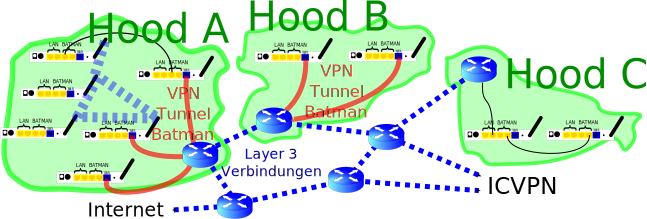
\includegraphics[width=\textwidth]{img/svg/freifunk_konzepte.pdf}

    Unser Freifunknetz ist in mehrere Layer-2 Inseln, die per Layer-3 miteinander verbunden sind,
    aufgeteilt. Die Hoods A und B in diesem Beispiel sind über unser VPN jeweise mit einem Router im
    Internet verbunden. Hood C hat einen lokalen Router, der direkt am LAN-Port hängt.
\end{frame}

\begin{frame}{Fastdstart.sh}
    \begin{itemize}
        \item Legt config von fastd sowie up/down scripts an
        \item Startet fastd
        \item Meldet sich beim VPN-KeyXchange an
        \item Lädt Liste mit Peers
        \item Refresht fastd
    \end{itemize}
\end{frame}

\begin{frame}{VPN-KeyXchange}
    \begin{itemize}
        \item Knoten Identifizierung über MAC, alternativ über Name
        \item Jeweils pro hood:
        \begin{itemize}
            \item Clients bekommen eine Liste aller Gateways
            \item Gateways bekommen eine Liste aller Clients+Gateways
        \end{itemize}
    \end{itemize}
\end{frame}
